%! TEX root = /home/simon/Documents/masterarbete/dagbok/main.tex
\documentclass[swedish, a4paper, 11pt]{report}


%%%%%%%%%%% LANGUAGE %%%%%%%%%%%

% For correct hyphenation in swedish
\usepackage[T1]{fontenc}

% For interpreting non-ASCII characters
\usepackage[utf8]{inputenc}

% International language support
% Fetches language from documentclass options. Most other packages do this as well
\usepackage{babel}


%%%%%%%%%%% FORMAL STUFF %%%%%%%%%%%

% Smaller margins
\usepackage[margin=2.5cm]{geometry}

% Fancy chapter headers
\usepackage{titlesec}
\titleformat{\chapter}{\normalfont\huge}{\thechapter.}{20pt}{\huge\it}

% Dates & time
\usepackage[yyyymmdd]{datetime} % Useful when referencing websites
\renewcommand{\dateseparator}{-} % ISO 8601 date format

% What to display in table of contents
\setcounter{tocdepth}{1}
\setcounter{secnumdepth}{2}

% Lists
\usepackage{enumerate} % Determines the style in which the counter is printed
\usepackage{enumitem} % Provides user control over the layout of the three basic list environments

% Citing & bibliography
\usepackage{csquotes} % For \enquote command for proper quotation marks, also biblatex recommends this
\usepackage[numbers]{natbib}


%%%%%%%%%%% GRAPHICS %%%%%%%%%%%

\usepackage{graphics,color,xcolor}

% Figures
\usepackage{epsfig} % Solves some problems in \includegraphics{<.eps-file>}
\usepackage{graphicx} % More options for \includegraphics
\usepackage{wrapfig} % Figure environment that lets text wrap around figure
\usepackage{float} % Figure placement
\usepackage{caption} % More options for \caption
\usepackage{subcaption} % Subfigures

% Tikz
\usepackage{tikz}
\usepackage{pgf,pgfplots} % Pgfplot
\pgfplotsset{compat=1.15}

% För alduslöv
\usepackage{pifont}


%%%%%%%%%%% PHYSICS %%%%%%%%%%%

% SI units
\usepackage{siunitx}
\DeclareSIUnit\clight{\text{$c$}} % redefine from c_0 to c
\DeclareSIUnit\byte{B}

% Physics macros
\usepackage{physics} % Defines lots of nice commands like \derivative, \norm, \evaluated, etc. It is recommended to use these as much as possible for nice spacing and readable LaTeX code.
\usepackage{braket} % Defines \bra, \ket, \braket, and \set
\usepackage{slashed} % For Feynman slash notation
\usepackage{simpler-wick} % Wick contractions (may require sty-file)
% \usepackage[compat=1.1.0]{tikz-feynman} % Feynman diagrams (has to be compiled with LuaTeX)
\usepackage{tensor} % Covariant index notation


%%%%%%%%%%% CODING %%%%%%%%%%%

% For nice code insertions
\usepackage{listings}
\definecolor{codegreen}{rgb}{0,0.6,0}
\definecolor{codegray}{rgb}{0.5,0.5,0.5}
\definecolor{codepurple}{rgb}{0.58,0,0.82}
\definecolor{backcolour}{rgb}{0.95,0.95,0.92}
\lstdefinestyle{mystyle}{
    backgroundcolor=\color{backcolour},   
    commentstyle=\color{codegreen},
    keywordstyle=\color{magenta},
    numberstyle=\tiny\color{codegray},
    stringstyle=\color{codepurple},
    basicstyle=\ttfamily\footnotesize,
    breakatwhitespace=false,         
    breaklines=true,                 
    captionpos=b,                    
    keepspaces=true,                 
    numbers=left,                    
    numbersep=5pt,                  
    showspaces=false,                
    showstringspaces=false,
    showtabs=false,
    tabsize=4
}
\lstset{style=mystyle}


%%%%%%%%%%% MATHEMATICS %%%%%%%%%%%

% AMS packages
\usepackage{amsmath,amsfonts,amsthm,amssymb}

% Theorem and proof environments
\iflanguage{swedish}{
    \newtheorem{theorem}{Sats}
    \newtheorem*{theorem*}{Sats}
    \newtheorem{proposition}{Proposition}
    \newtheorem*{proposition*}{Proposition}
    \newtheorem{corollary}{Följdsats}[theorem]
    \newtheorem{corollary*}{Följdsats}
    \newtheorem{lemma}{Lemma}
    \newtheorem*{lemma*}{Lemma}
    \theoremstyle{definition}
    \newtheorem{definition}{Definition}
    \newtheorem*{definition*}{Definition}
}{}
\iflanguage{english}{
    \newtheorem{theorem}{Theorem}
    \newtheorem*{theorem*}{Theorem}
    \newtheorem{proposition}{Proposition}
    \newtheorem*{proposition*}{Proposition}
    \newtheorem{corollary}{Corollary}[theorem]
    \newtheorem{corollary*}{Corollary}
    \newtheorem{lemma}{Lemma}
    \newtheorem*{lemma*}{Lemma}
    \theoremstyle{definition}
    \newtheorem{definition}{Definition}
    \newtheorem*{definition*}{Definition}
}{}

% Better version of the \not command
\usepackage{cancel}

 % Does polynomial division for you
\usepackage{polynom}

% Vectors are upright boldface. I think this definition is better than the physics package's \vectorbold.
\let\Vec\undefined % We use \vec w/ lowercase v
\renewcommand*{\vec}[1]{{\boldsymbol{\mathrm{#1}}}}

% Bar, tilde, and hat that scales with what is under them. Basically I just want these to have consistent names
\let\mathbar\overline
\let\mathtilde\widetilde
\let\mathhat\widehat

% Redefine \exp
% Errors occur if this definition is made before some of the packages are loaded
\let\oldexp\exp
\newcommand*{\Exp}[1]{\oldexp{#1}}
\renewcommand{\exp}[1]{\mathrm{e}^{#1}}

% Main number systems
\newcommand{\naturals}{\mathbb{N}}
\newcommand{\integers}{\mathbb{Z}}
\newcommand{\rationals}{\mathbb{Q}}
\newcommand{\reals}{\mathbb{R}}
\newcommand{\compexnumbers}{\mathbb{C}}

% Some of my own shorthands for correct spacing in math environments
\def\divides{\mid} % Proper spacing of vertical bar in division x|y
\def\from{\colon} % Proper spacing of colon in functions f:A→ B
\newlength\mylen % Isomorphic \mapsto
\settowidth\mylen{$\longleftrightarrow$}
\newcommand{\mapsbetween}{\longleftrightarrow\kern - 0.5\mylen\vline height 1.2ex depth -0.0pt\kern0.5\mylen}
\newcommand{\suchthat}{\qq{s.th.}}
\def\definedas{\coloneqq}
\def\defines{\eqqcolon}

\newcommand*{\transpose}[1]{#1^{\!\mathsf{T}}}
\renewcommand*{\complement}[1]{#1^{\mathsf{C}}}
% \newcommand{\conjugate}[1]{\mathbar{#1}}
\newcommand*{\conjugate}[1]{#1^*}
\newcommand*{\hermitianconjugate}[1]{#1^\dag}
\newcommand*{\inverse}[1]{#1^{-1}}

\newcommand*{\closure}[1]{\mathbar{#1}} % Closure of a set
\def\union{\cup}
\newcommand{\Union}{\bigcup\limits}
\def\intersection{\cap}
\newcommand{\Intersection}{\bigcap\limits}

% Lie-groups & algebras, i.g. SU(n)
\newcommand*{\algebra}[2]{\mathfrak{\MakeLowercase{#1}}\left(#2\right)}
\newcommand*{\group}[2]{\mathrm{\MakeUppercase{#1}}\left(#2\right)}


%%%%%%%%%%% MISCELLANEOUS %%%%%%%%%%%

% In-pdf comments through \todo command
\setlength{\marginparwidth}{2cm} % Silence warning about margin size
\usepackage{todonotes}

% Clickable links and refs
\usepackage[hidelinks]{hyperref} 

% Cleverref automatically detects if you are referencing a figure, table, or equation etc
% Cleverref has to be loaded last I think, after babel and hyperref etc
\usepackage[noabbrev, nameinlink]{cleveref}
\crefname{equation}{}{}
\iflanguage{swedish}{ % Tell cleverref to use Oxford comma
	\newcommand{\creflastconjunction}{, och\nobreakspace}
}{}
\iflanguage{english}{
	\newcommand{\creflastconjunction}{, and\nobreakspace}
}{}


% Tag only referenced equations (this is not an ideal package, as it requires etextools, which is buggy and abandoned by its author)
\expandafter\def\csname ver@etex.sty\endcsname{3000/12/31}
\let\globcount\newcount
\usepackage{autonum}

% Intervals on the real line
\let\interval\undefined % To avoid name conflict with etextools
\usepackage{interval}
\intervalconfig{soft open fences}

% For writing \overset{text}&{=} in align environment
\usepackage{aligned-overset} 

\begin{document}


\section*{Code insert}
\lstinputlisting[language=C]{templates/kahan_summation_algorithm.c}


\section*{subfigures}
\begin{figure}[H]
    \centering
    \begin{subfigure}{.5\linewidth}
        
\includegraphics[width=\textwidth]{templates/osmium.jpg}
        \caption{}
        \label{fig:a}
    \end{subfigure}%
    \begin{subfigure}{.5\linewidth}
        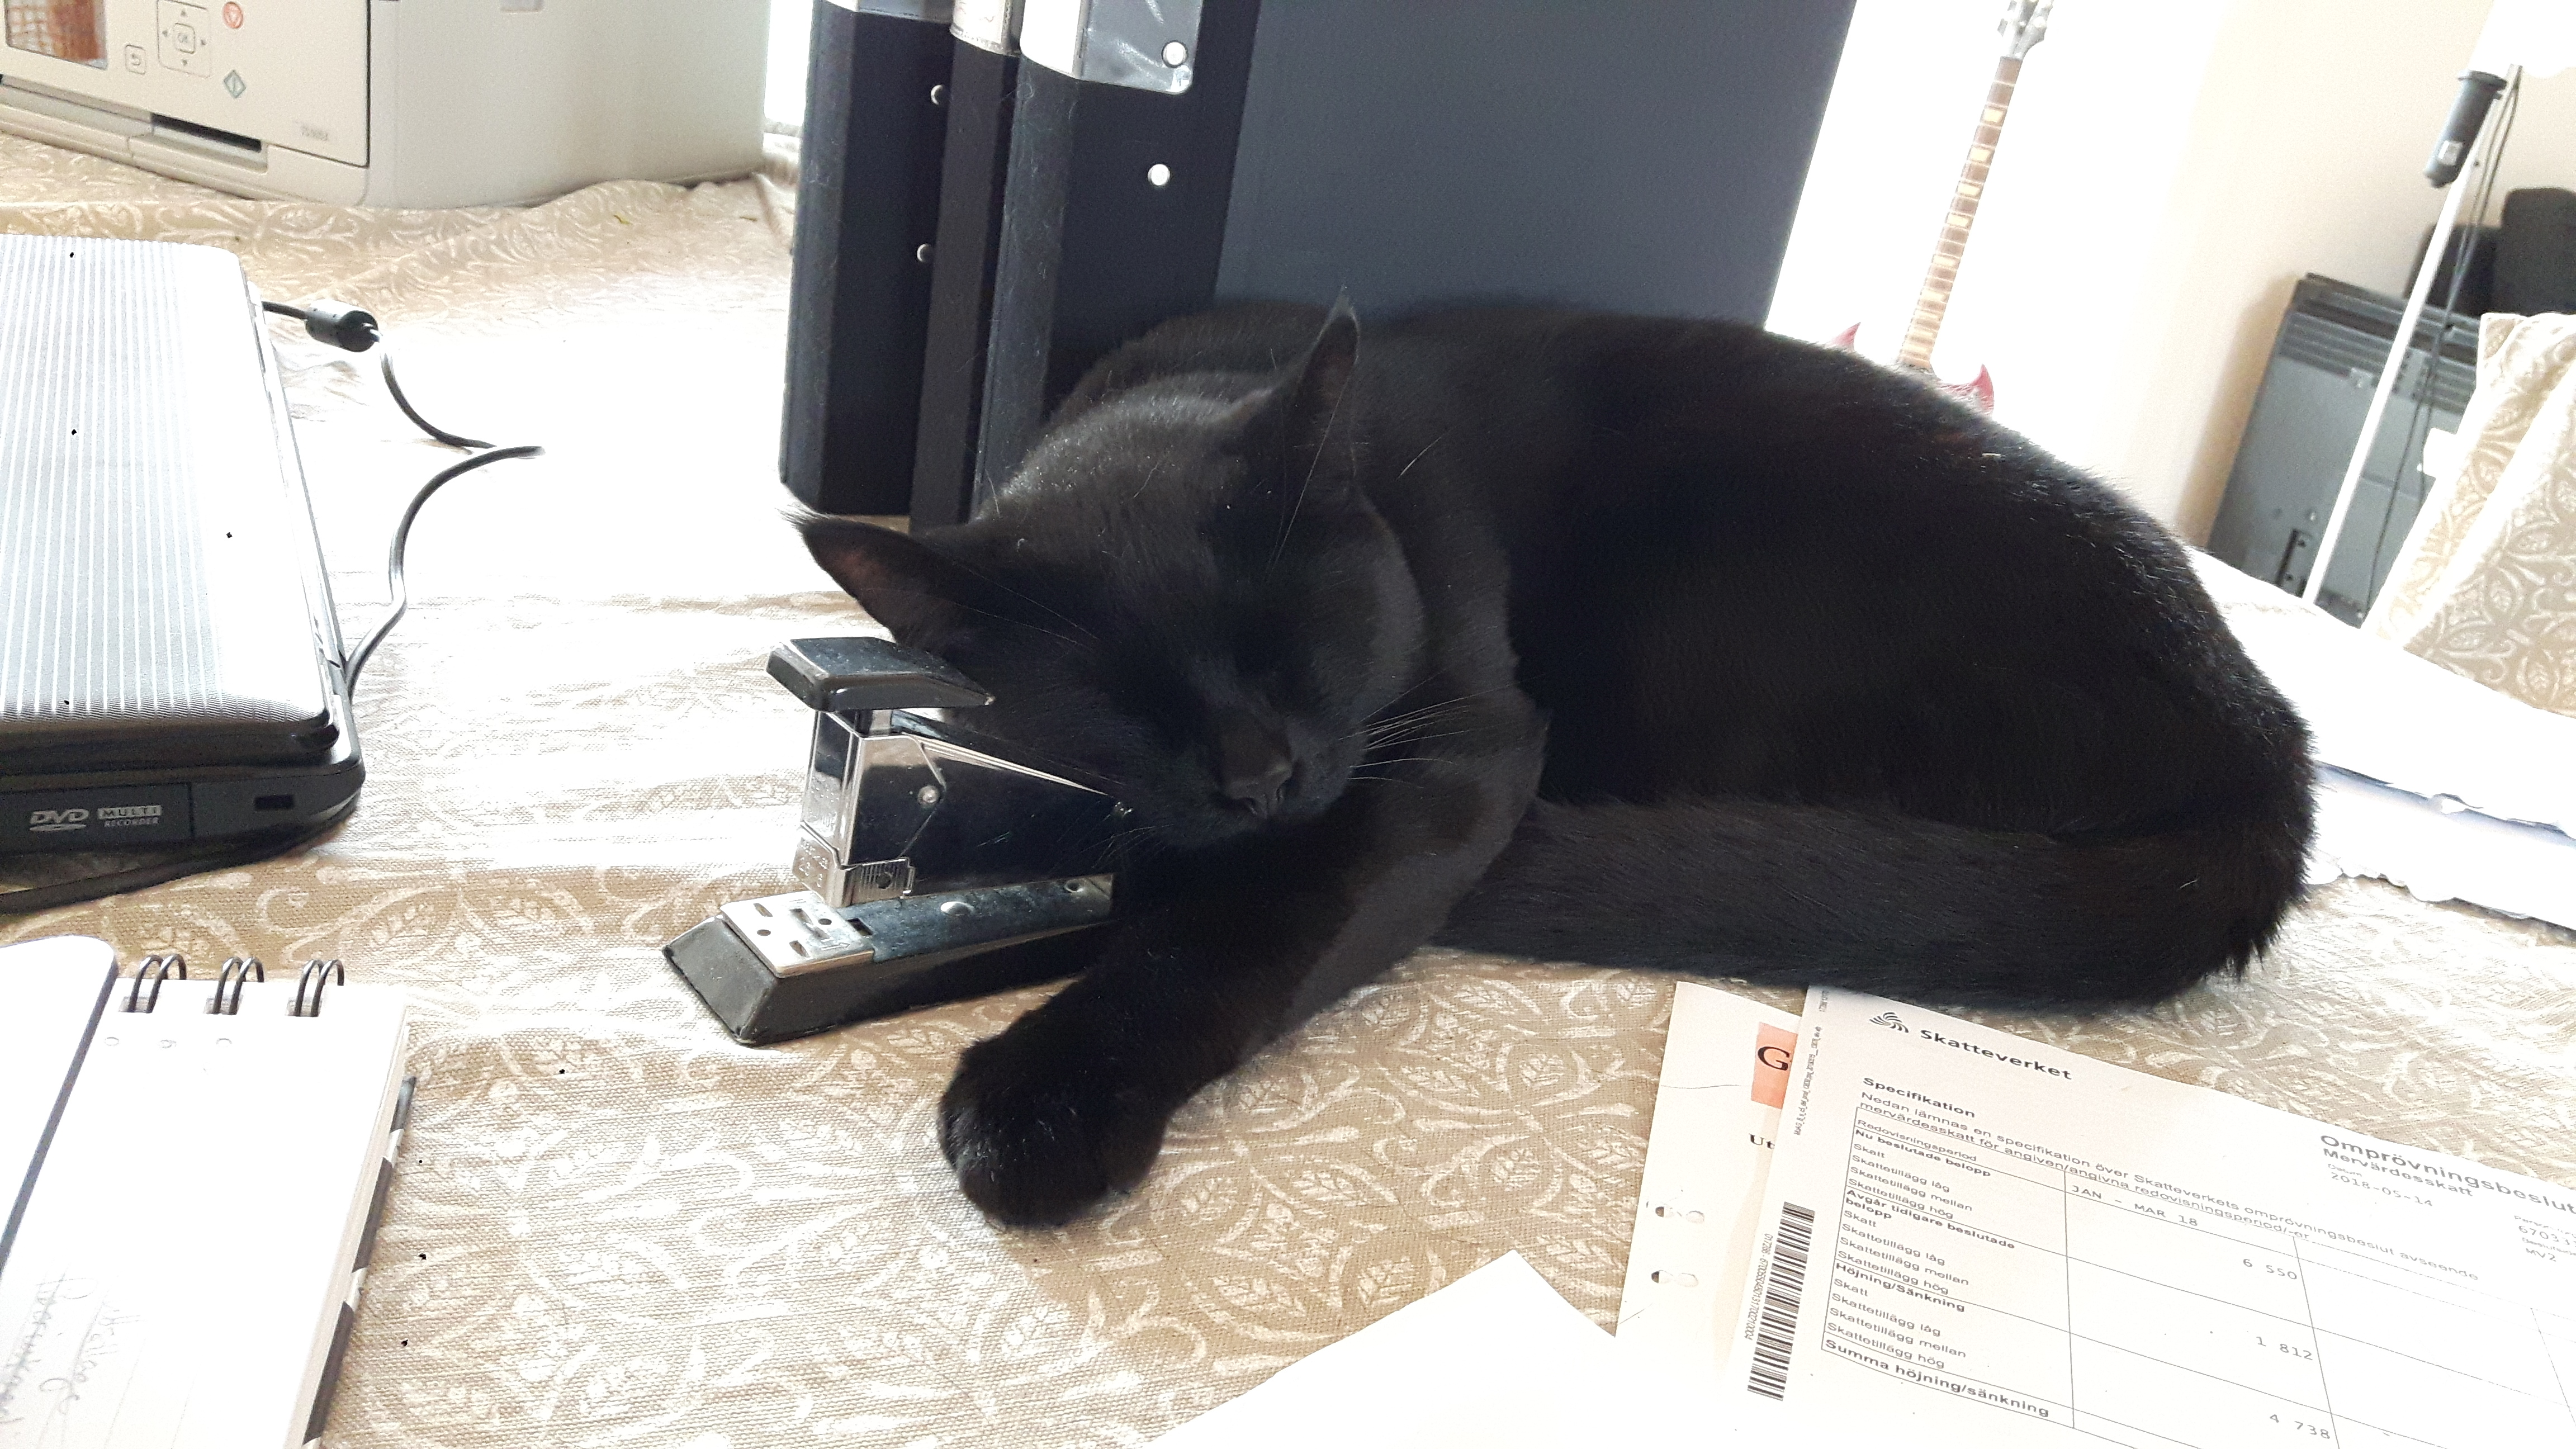
\includegraphics[width=\textwidth]{templates/murre.jpg}
        \caption{}
        \label{fig:b}
    \end{subfigure}
    \caption{}
\end{figure}


\section*{Tikz figure}
\begin{figure}[H]
    \centering
    \begin{tikzpicture}
            % Coordinate axii
            \draw[-latex,black] (-3,0) -- (3,0) {};
            \draw[-latex,black] (0,-3) -- (0,3) {};
            
            % Vector arrows
            \draw[-latex,black,thick] (0,0) -- (2,0) node[label=90:$\alpha$] {};
            \draw[-latex,black,thick] (0,0) -- (-1,1.73205) node[label=180:$\beta$] {};
            
            % Place some circles
            \filldraw[color=black, fill=white] (0,0) circle (4pt);
            \filldraw[color=black, fill=white] (0,0) circle (2pt);
            
            \filldraw[color=black, fill=white] (-1, -1.73205) circle (2pt);
            \filldraw[color=black, fill=white] (1, 1.73205) circle (2pt);
            \filldraw[color=black, fill=white] (1, -1.73205) circle (2pt);
            \filldraw[color=black, fill=white] (-2, 0) circle (2pt);
    \end{tikzpicture}
    \caption{}
    \label{fig:}
\end{figure}


\section*{Mulitline text equations}
This is a quote:
\begin{quote}
    For every connected domain $V$ that intersects the boundary $\partial \Omega$ and for every component $V_i$ of $V \cap \Omega$, there is a function $f \in \mathcal{O}(\Omega)$ whose restriction $f|_{V_i}$ has no direct analytic continuation to $V$.
\end{quote}{}
This is an equation with parbox:
\begin{equation}\label{eq:statement_that_Omega_is_domain_of_holomorphy}
    \parbox{0.85\textwidth}{
        For every connected domain $V$ that intersects the boundary $\partial \Omega$ and for every component $V_i$ of $V \cap \Omega$, there is a function $f \in \mathcal{O}(\Omega)$ whose restriction $f|_{V_i}$ has no direct analytic continuation to $V$.
    }
\end{equation}{}
They look basically the same, but I use the latter one so that I can ref it like this \cref{eq:statement_that_Omega_is_domain_of_holomorphy}.


\section*{Cite}
For learning about quantum computing, see \cite{Nielsen:2011}.

If we want to know what Planck's constant divided by Planck's reduced constant is, we can plug \enquote{(plancks constant) / (plancks reduced constant)} into Wolfram Alpha and get $2 \pi$ \cite{Wolfram|Alpha}.

The speed of light is, according to my physics handbook, \SI{2.99792458e8}{\meter \per \second} \cite{Physics_handbook}.



\newpage
\appendix
\printbibliography

\end{document}